% LTeX: language=de-DE
\chapter{Mechanik}
	Wie in \cref{sec:constructive limitations} besprochen beschränkt sich die Auswahl möglicher Antriebselemente praktischerweise auf BLDC-Motoren die wiederum auf dem Markt als \textit{Inrunner} und \textit{Outrunner} erhältlich sind.
	In ersteren sind die Statorwicklungen an der Außenseite angeordnet, zweitere ordnen sie an der Innenseite an.
	\begin{figure}[h]
		\centering
		\includesvg[width=.8\textwidth]{Assets/Inrunner_Outrunner}
		\caption[Gegenüberstellung von Inrunner und Outrunner]{Schematische Gegenüberstellung von BLDC-Motoren als Inrunner (links) bzw. Outrunner (rechts) ausgeführt~\cite{inrunner.outrunner.2022}.}
		\label{fig:inrunner outrunner}
	\end{figure}
	Das Funktionsprinzip bleibt so zwar unverändert, durch den vergrößerten Radius des Angriffspunktes der magnetischen Kopplung kann bei gleicher Baugröße und gleichem Phasenstrom allerdings ein höheres Drehmoment erzeugt werden.
	Sind größere Drehzahlen gefordert, so ist die Bauweise des Inrunners durch den reduzierten Durchmesser des Rotors vorteilhaft.
	Da hohe Drehzahlen gegenüber einem zu erzeugenden Drehmoment für das zu konstruierende Antriebssystem von untergeordneter Priorität sind und sich oberhalb eines Schwellwertes sogar kontraproduktiv auswirken können fällt hier die Wahl auf das Outrunnerprinzip.\par\medskip
	%
	Auch während Lenkmanövern muss eine Übertragung des Drehmomentes auf die Rollen der Trucks sichergestellt sein.
	Praktikabel und mit einfachen Mitteln denkbar sind hier eine koaxiale Positionierung des Motors zur angetrieben Rolle.
	Der Motor kann hier unter eines Offsets weiter im Zentrum des Hangers platziert werden, setzt in dem Fall jedoch eine Hohlwelle zwingend voraus.\par
	Eine weitere Option bildet die Positionierung des Motors in der Rolle selbst.
	Beschichtet mit einem geeigneten Material kann der Rotor so unmittelbar den Kontakt zum Boden herstellen.
	Vorteile dieser Variante sind sowohl eine gute Marktverfügbarkeit, als auch eine deutliche Reduktion mechanischer Komplexität des Antriebssystems.
	Nachteilig sind hier im Vergleich deutlich höhere Preise, weniger Auswahl und schlechte Wartungsmöglichkeiten.\par
	Letztlich kann die Motorachse parallel zur Rollenachse positioniert werden.
	So ist zwar die Kraftübertragung von Welle zu Rolle aufwändiger herzustellen, es werden aber die geringsten Anforderungen an die Motoren bezüglich ihrer Bauform gestellt wodurch sie besonders günstig und in großer Vielfalt am Markt verfügbar sind.\par\medskip
	%
	Gegenüber BLDC-Motoren, die etwa für den Bau von Drohnen für besonders hohe Drehzahlen optimiert sind, steht in der vorliegenden Anwendung das erreichbare Drehmoment im Vordergrund.
	
	Als praktikabel hat sich der Motor mit Handelsnamen \textit{TorqueBoards} und der Typenbezeichnung \textit{6355 190KV} gezeigt.
	Die äußeren Dimensionen können \cref{fig:motor} entnommen werden\footnote{Eigene Zeichnung mangels technischer Zeichnungen seitens des Herstellers.
	Alle Dimensionen wurden der Produktbeschreibung entnommen oder wo fehlend messtechnisch ergänzt.}.
	\begin{figure}[h]
		\centering
		\includesvg[width=.9\textwidth]{Footage/AwesomeBoard Transmission CAD/Drawings/Motor}
		\caption{Relevante Dimensionen des Motors \textit{TorqueBoards 6355 190KV}.}%
		\label{fig:motor}
	\end{figure}
	%
	\section{Transmission}\label{sec:transmission}
		Um das Drehmoment von der Motorwelle auf die Rolle zu übertragen wurde ein Riemensystem mit \textit{High Torque Drive}-Profil (HTD\nomenclature[A]{HTD}{High Torque Drive}) in Zahnteilung 5M gewählt. 
		Seine vergleichsweise breite Zahnung bietet einen guten Kompromiss aus Flexibilität, Kraftübertrag und Effizienz \cite{gates.catalogue.2021}.
		Darüber hinaus sind entsprechende Riemen und Zahnscheiben günstig und gut erhältlich.\par\medskip
		%
		Um eine gegebenenfalls notwendige Untersetzung abzuschätzen, kann der Quotient aus \cref{eq:frictionless torque} und \cref{eq:incline torque} als Funktion von \(\zeta\) aufgetragen werden.
		Erwünscht ist hier ein Wert \(\gg 1\), mindestens aber \(= 1\).
		\begin{equation}
			\frac{T}{T_{Hang}} = \frac{8,27 \cdot I_{Motor} \cdot \zeta}{K_V \cdot m \cdot g \cdot \sin\left(\arctan\left(\frac{\angle}{\qty{100}{\percent}}\right)\right)}
			\label{eq:torque ratio}
		\end{equation}
		Daneben soll auch die erwartete Maximalgeschwindigkeit nach \cref{eq:max speed km h} abgeschätzt werden.
		Einsetzen der bekannten Parameter und Randbedingungen aus \cref{sec:constructive limitations} in \crefrange{eq:torque ratio}{eq:max speed km h} im Intervall \(1 \leq \zeta \leq 3\) ist in \cref{fig:torque ratio and vmax vs zetas} dargestellt.
		Zu sehen ist, dass mindestens \(\zeta \approx 1,5\) erreicht werden muss um die Vorgaben erfüllen zu können.
		Da die Maximalgeschwindigkeit hier aber mit nahe \qty{70}{\kilo\metre} für die Anwendung deutlich zu hoch liegt, wird \(\zeta \approx 2,5\) gewählt.
		\begin{figure}[h]
			\centering
			\includesvg[width=.85\textwidth]{Calc/T_v_vs_zetas}
			\caption{Plot}
			\label{fig:torque ratio and vmax vs zetas}
		\end{figure}
		
		Da im Falle der HTD 5M Zahnung gilt, dass zu jedem Zeitpunkt zumindest sechs Zähne greifen müssen~\cite{MAEDLERGmbH.2021} und mit obigen Überlegungen die antriebsseitige Zahnscheibe kleiner gegenüber der getriebeseitigen sein muss, ergibt sich eine antriebsseitige Mindestzahnung.
		Da mit dem gewählten Untersetzungsverhältnis sich die Zahnung auch auf die der Antriebsseite und damit den äußeren Durchmesser auswirkt
		Dieser darf den Durchmesser der Rolle abzüglich des zusätzlichen Auftrags des Riemens von \qty{1,7}{\milli\metre}\cite{gates.catalogue.2021} nicht übersteigen, um im Betrieb Bodenkontakt des Riemens zu vermeiden.
		Während käuflich Zahnungen von 12 an aufwärts gelistet sind, bot sich aus Kostengründen eine Variante mit 15 Zähnen an.
		Gerundet auf \(\zeta=2,4\) ergibt sich so eine Zahnung von 36 für die Getriebeseite.
		
		Da auf der getriebenen Seite die Zahnscheibe kraftschlüssig mit der Rolle verbunden werden muss ist es wünschenswert, dass sich durch die Bauart der Rollen bereits eine einfache Installation anbietet.
		Verwendet werden hier \qty{80}{\milli\metre} \textit{Kegel} des Herstellers \textit{Orangatang}.
		Sie besitzen einen Kern aus hartem Kunststoff mit 10 radial um ihre Hauptachse angeordneten Bohrungen von \qty{5,8}{\milli\metre} Durchmesser (vgl. \cref{fig:kegels}).
		\begin{figure}[h]
			\centering
			\includesvg[width=.8\textwidth, inkscapelatex=false]{Footage/AwesomeBoard Transmission CAD/Drawings/Orangatang Kegel 83mm Longboard Wheel}
			\caption[Rück- und Schnittansicht der \textit{Kegel} des Herstellers \textit{Orangatang}]{Rück- und Schnittansicht der \textit{Kegel} des Herstellers \textit{Orangatang}. Die Zahnscheibe wird rückseitig auf der Rolle montiert.}
			\label{fig:kegels}
		\end{figure}

		Aus Kostengründen und einfachem Zugang zu den Betriebsmitteln wurde sich entschieden, die getriebeseitige Zahnscheibe im FDM-Verfahren\nomenclature[A]{FDM}{Fused Deposition Modeling} aus ABS selbst herzustellen.
		Es ist zwar zu erwarten, dass die Zahnscheiben gegenüber aus Aluminium gefrästen Komponenten deutlich schneller verschleißen, durch das gewählte Fertigungsverfahren lassen sich aber schnell, unkompliziert und günstig Ersatzteile herstellen.
		\begin{figure}[h]
			\centering
			\includesvg[width=.9\textwidth, inkscapelatex=false]{Footage/AwesomeBoard Transmission CAD/Drawings/HTD Parametric Pulley}
			\caption[Zeichnung der modellierten Zahnscheibe]{Zeichnung der modellierten Zahnscheibe. Zu erkennen sind alternierend fünf Bohrungen um jeweils M4 Schrauben aufnehmen zu können und fünf Führungsstifte für eine vereinfachte Montage.}
			\label{fig:htd 5m driven}
		\end{figure}

		Unter Zuhilfenahme einer Fühlerlehre, ermitteln der Maße und mehreren Iterationen 3D-gedruckter Modelle konnten die inneren Profile der Rollen in ausreichender Genauigkeit so in ein CAD-Modell übertragen werden, dass daraus eine Passung für die getriebeseitige Zahnscheibe modelliert werden kann.
		Das Zahnungsprofil wurde aus einem OpenSCAD-Script\cite{thingiverse.tooth.profiles.2012} entnommen, um es unter Abgleich von Herstellerangaben\cite{gates.catalogue.2021,GatesCorporation.drive.design.manual.2014} im verwendeten CAD-Programm\footnote{Hier SolidWorks.} nachzubilden.
		Das Produkt ist die in \cref{fig:htd 5m driven} gezeigte Zahnscheibe mit 36 Zähnen.
		Korrespondierend mit den vorhandenen Bohrungen der Rollen umgibt das zentrale Loch fünf Bohrungen mit Senkung um DIN 912 M4 Schrauben aufnehmen zu können.
		Die in den Zwischenräumen angeordneten Stifte dienen nicht der Kraftübertragung, sondern lediglich einer einfacheren Montage.
		
		Wie in \cref{fig:HTD profiles comparison} zu sehen ist die Passform des Zahnungsprofils im direkten Vergleich zu einem Kaufteil (hier mit 44 Zähnen) hinreichend genau.
		Das Herstellungsverfahren lässt zwar etwas höhere Präzision zu, da aber im Betrieb ohnehin von abrasiven Effekten entlang der Zahnung ausgegangen wird, wurde im Sinne einer zügigeren Fertigung darauf verzichtet.
		\begin{figure}[h]
			\centering
			\begin{subfigure}{.49\textwidth}
				\centering
				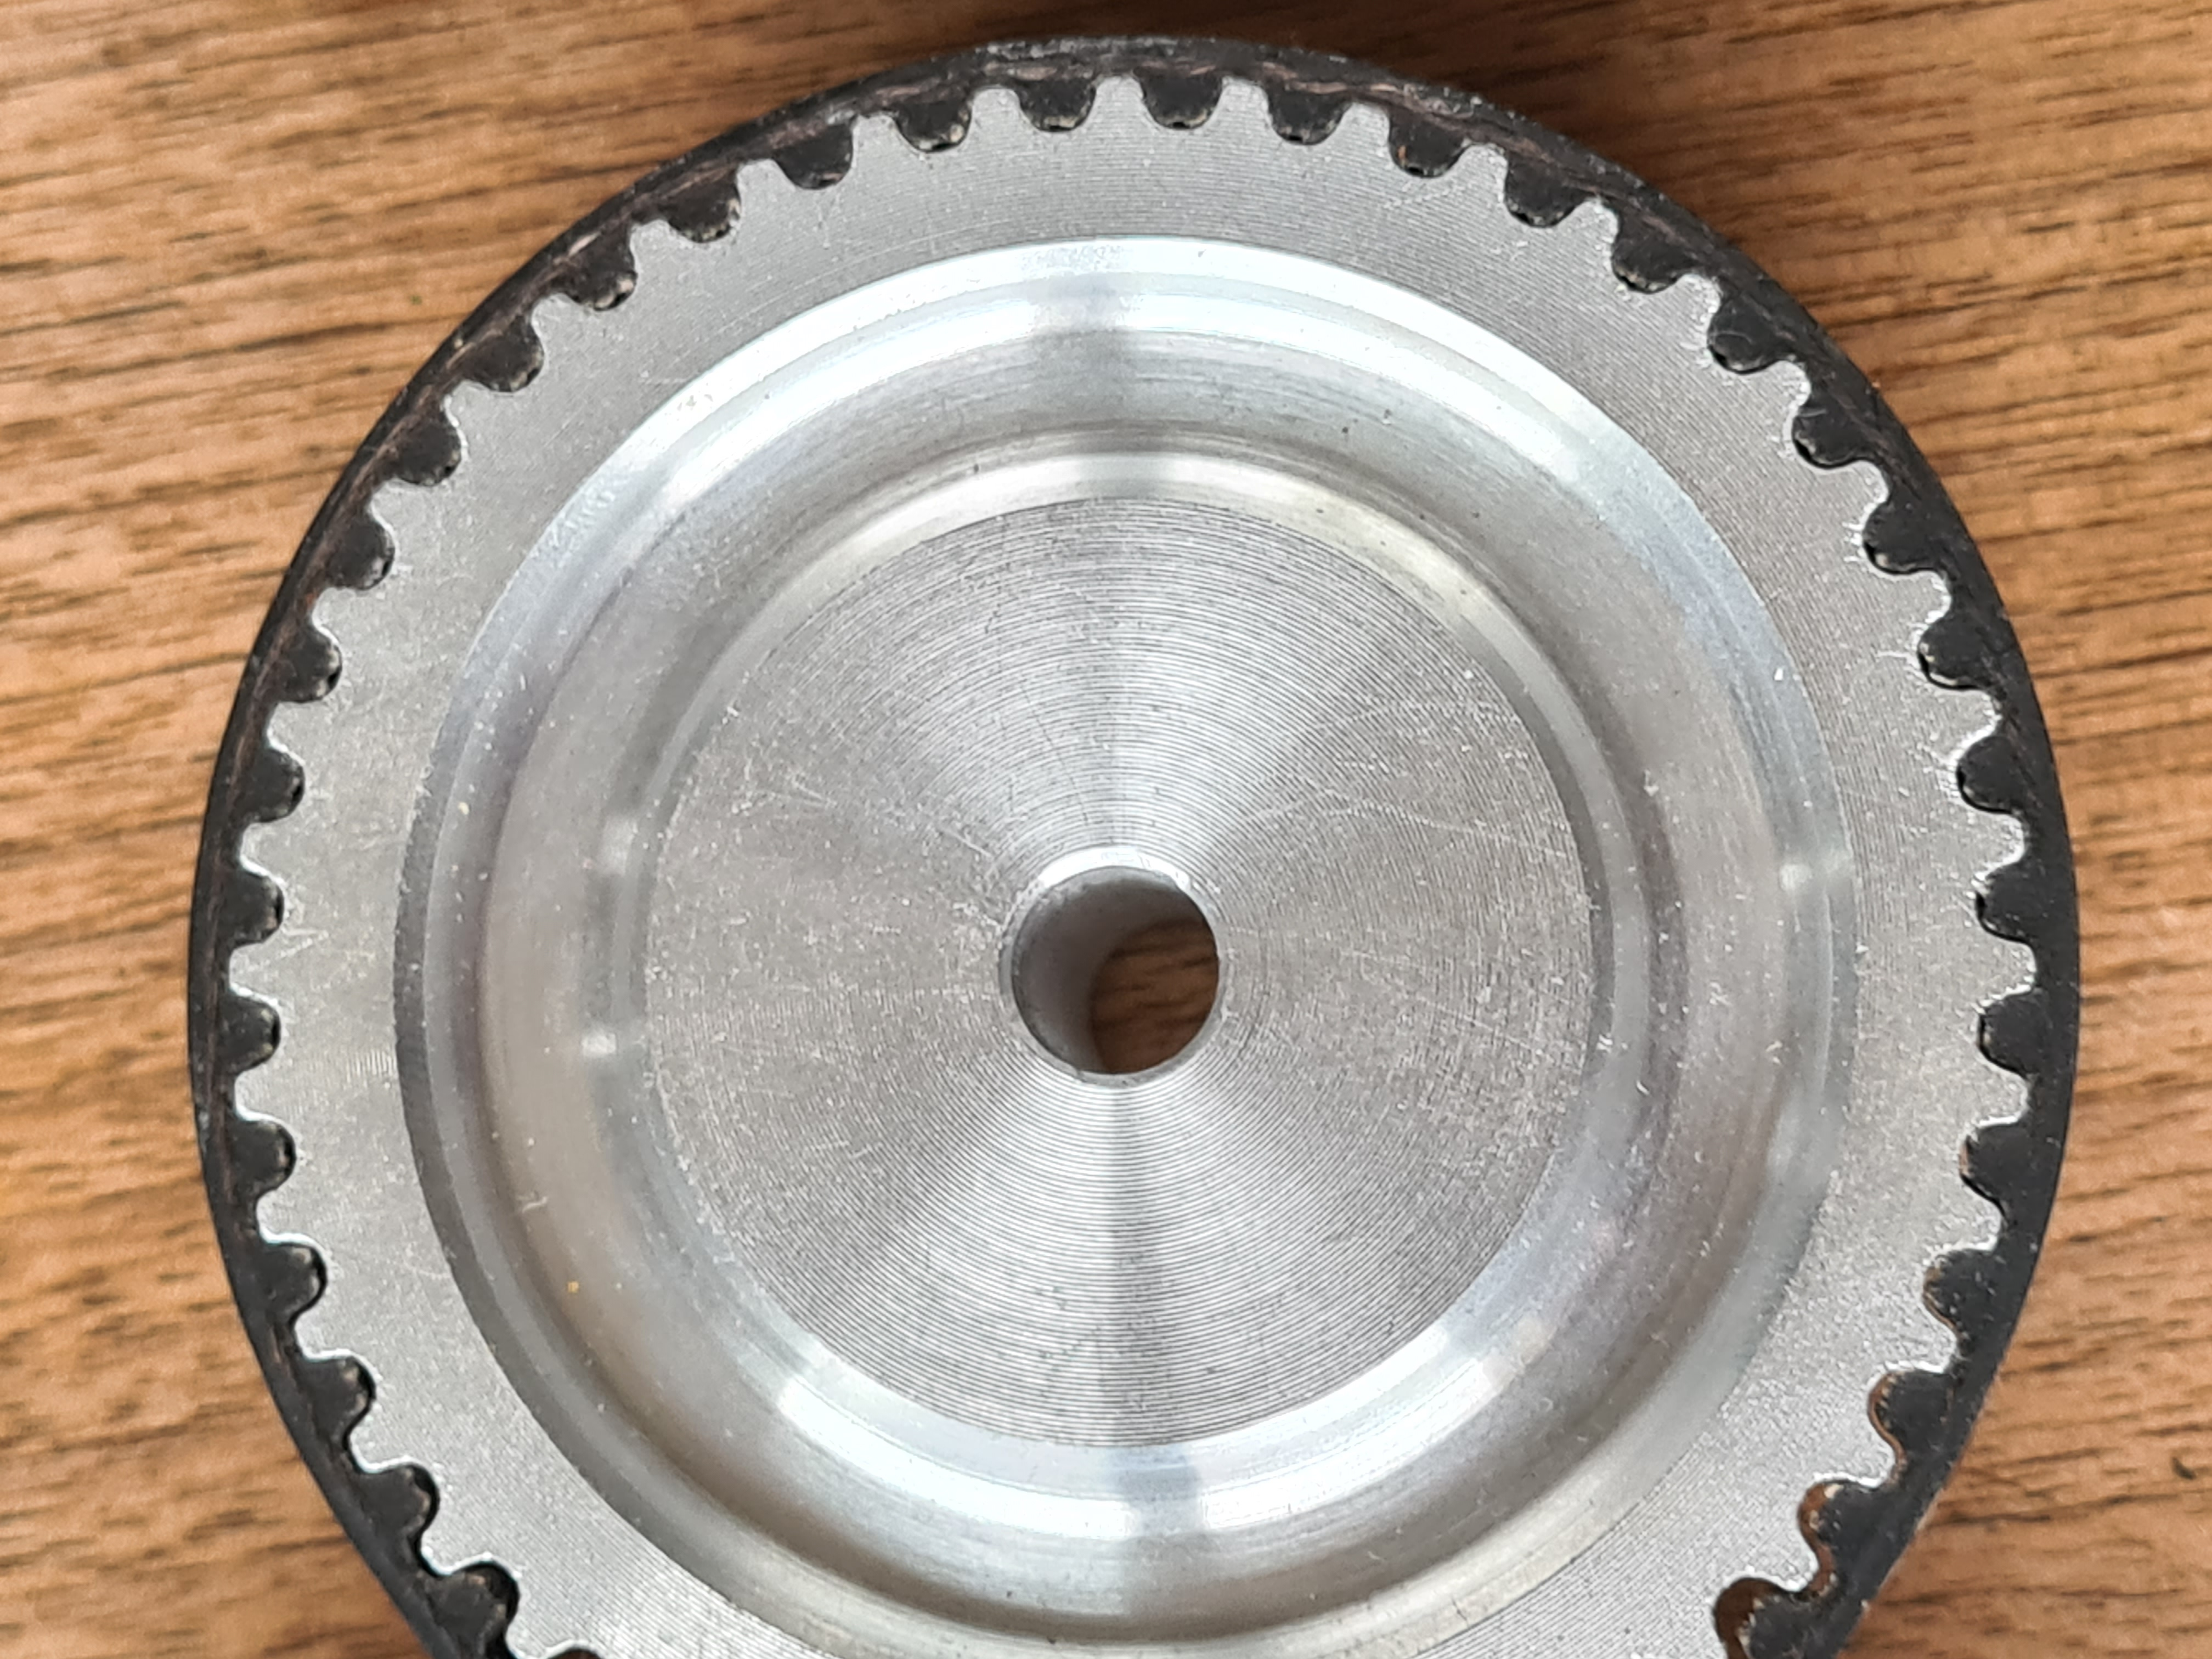
\includegraphics[width=\textwidth]{Assets/Machined-HTD_tooth_fit.jpg}
				\caption{CNC-gefrästes HTD-Profil auf Riemen.}
				\label{subfig:machined HTD}
			\end{subfigure}
			\hfill
			\begin{subfigure}{.49\textwidth}
				\centering
				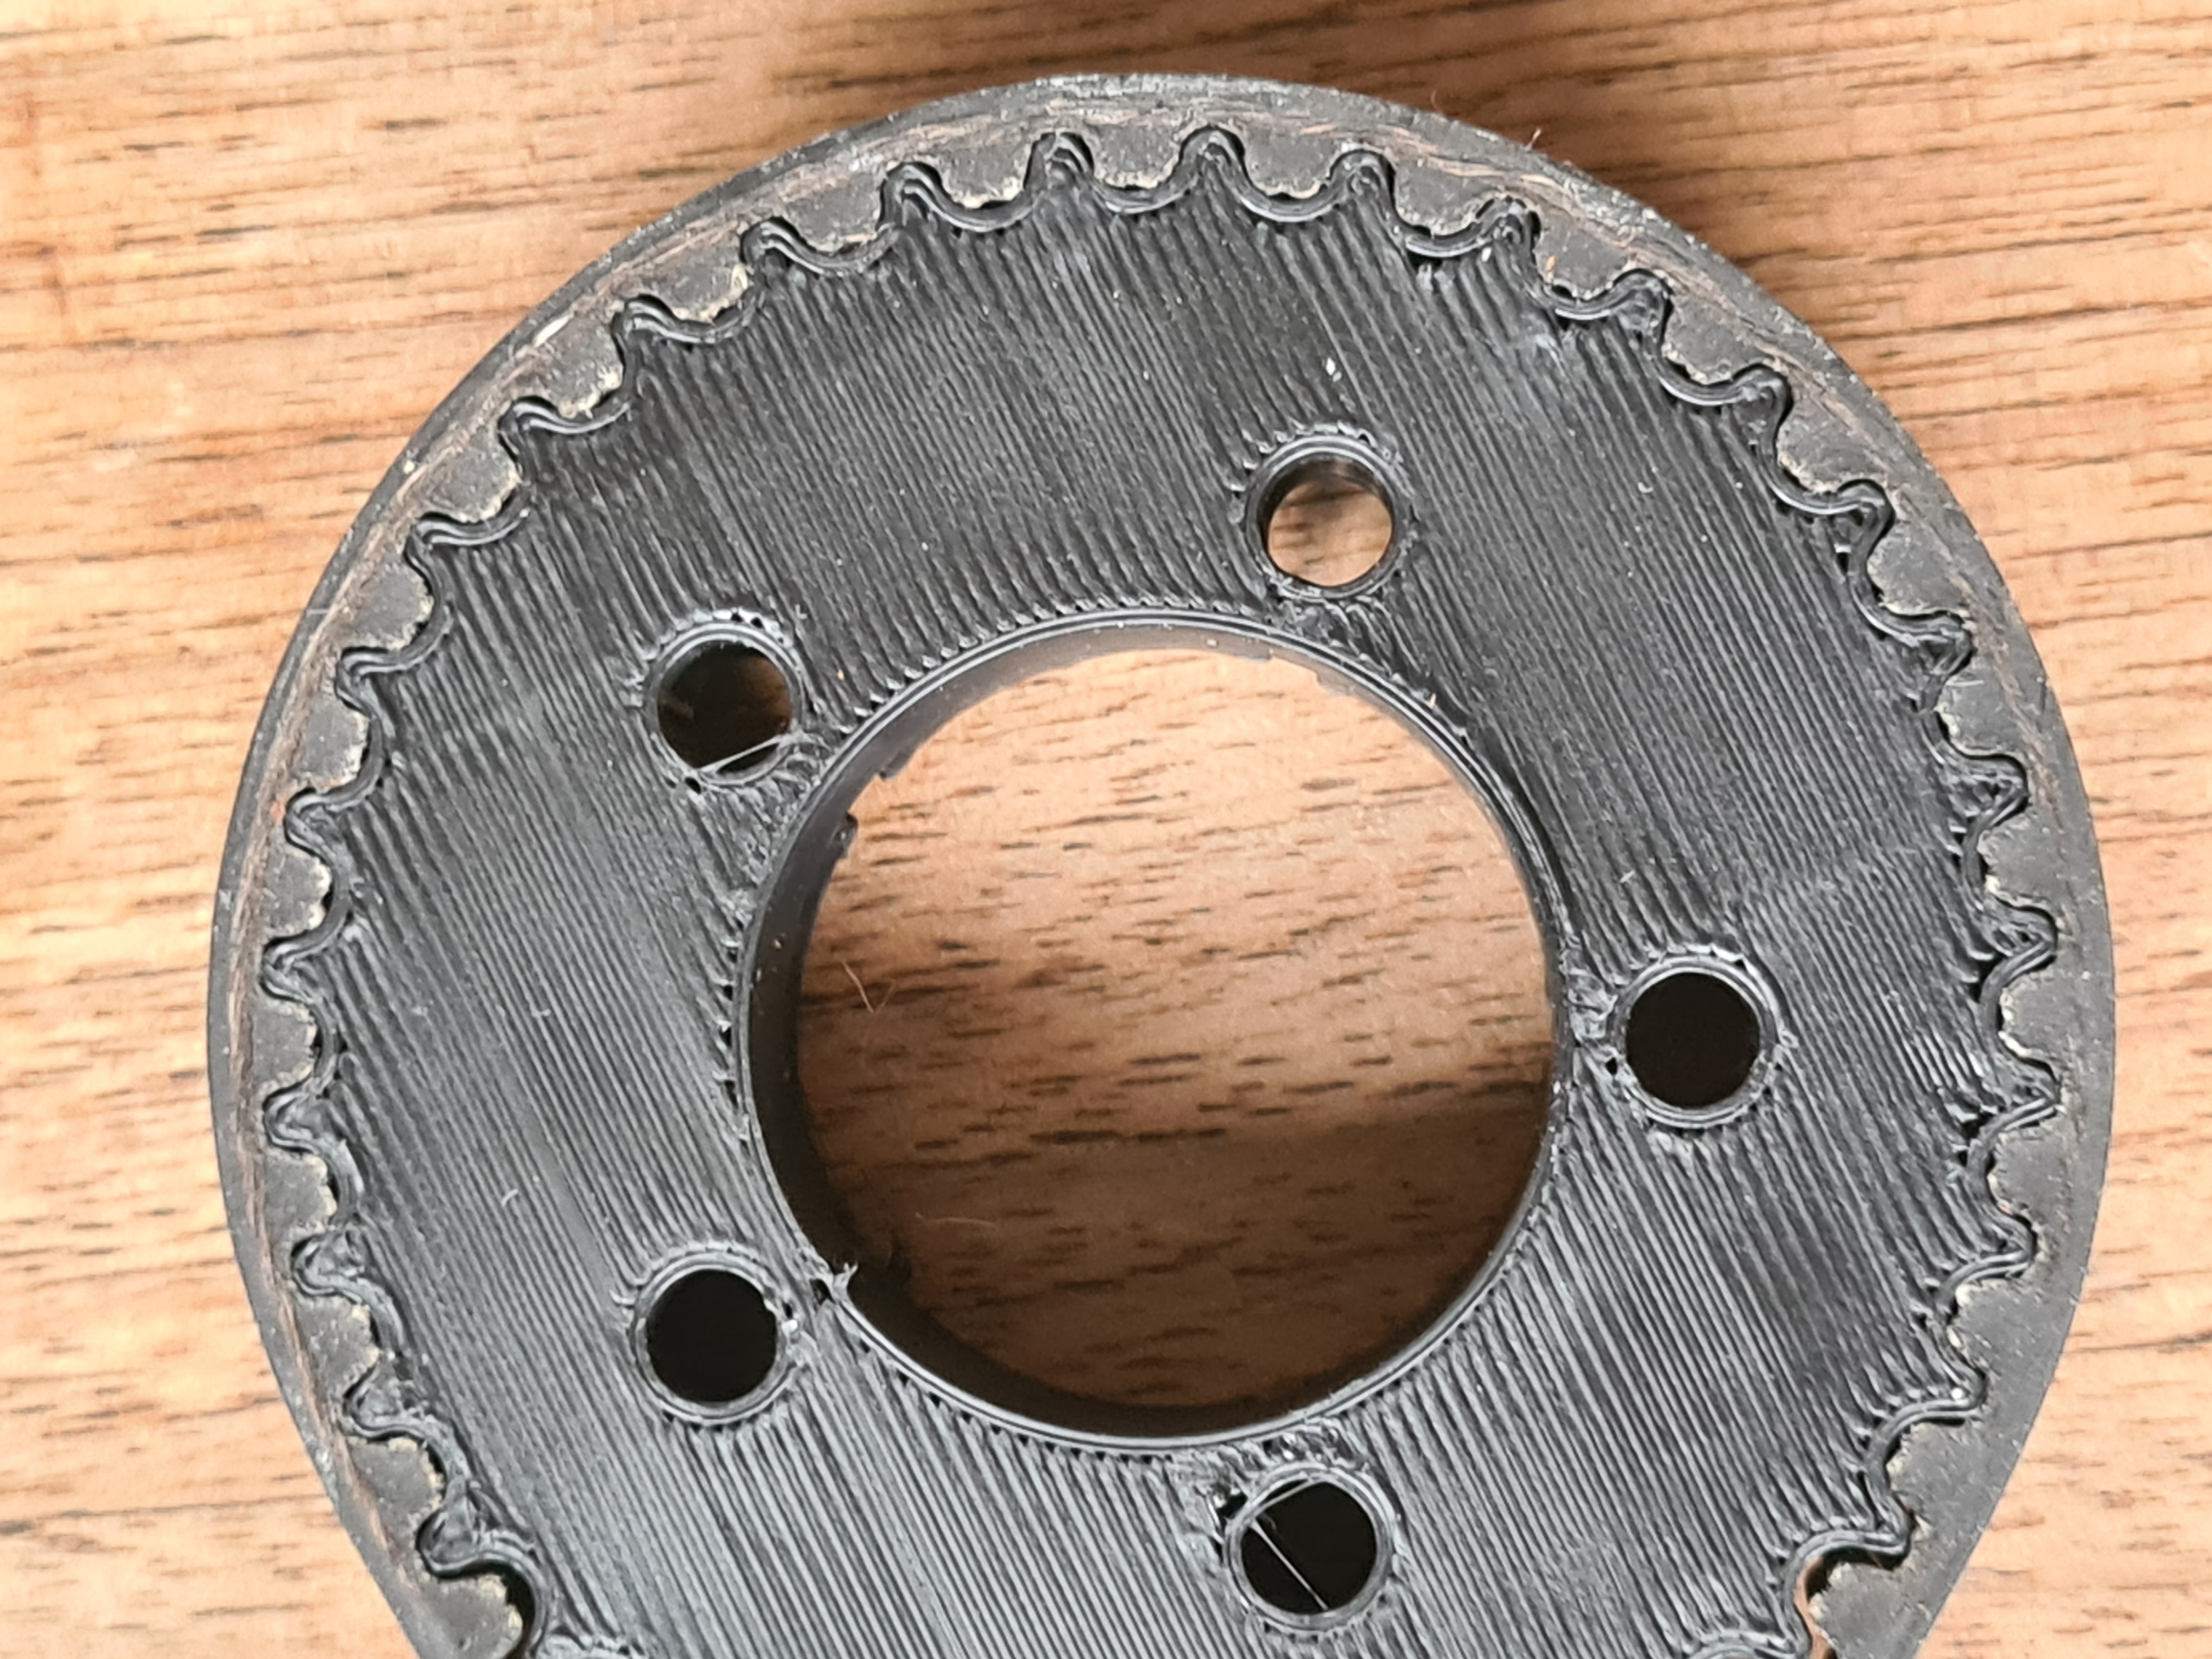
\includegraphics[width=\textwidth]{Assets/Printed-HTD_tooth_fit.jpg}
				\caption{3D-gedrucktes HTD-Profil auf Riemen.}
				\label{subfig:printed HTD}
			\end{subfigure}
			\caption{Vergleich der Passform einer gekauften Zahnscheibe (44T) aus Aluminium und des 3D-gedruckten Modells (36T) mit einem Riemen.}
			\label{fig:HTD profiles comparison}
		\end{figure}\par\medskip
		%
		Da die Schrauben mit Muttern gekontert werden sollen und die der Zahnscheibe gegenüberliegende Seite der Rollen ebenfalls ein konkaves Profil aufweist wurde ein komplementäres Gegenstück -- zu sehen in \cref{fig:orangatang kegel flat face} -- modelliert.
		\begin{figure}[h]
			\centering
			\includesvg[width=.5\textwidth, inkscapelatex=false]{Footage/AwesomeBoard Transmission CAD/Drawings/Orangatang Kegel Flat Face}
			\caption[Zeichnung des Gegenstücks der Zahnscheibe]{Zeichnung des Gegenstücks der Zahnscheibe um eine ebene Fläche für die Muttern zur Verfügung zu stellen.}
			\label{fig:orangatang kegel flat face}
		\end{figure}
		Wie auch die Zahnscheibe enthält die Konterscheibe fünf Bohrungen und fünf Führungsstifte und soll möglichst exakt dem inneren Profil der Rollen anliegen.
		Da die Konterscheibe durch die Verschraubung gegen das Rollenprofil verspannt wird, ist eine gute Passgenauigkeit hier insbesondere wichtig um die Last über die gesamte Fläche zu verteilen und so die Gefahr frühzeitigen und/oder plötzlichen Materialversagens vorzubeugen.

		Ein vergrößerter Mittelpunktabstand beider Zahnscheiben erhöht grundsätzlich die Anzahl greifender Zähne, allerdings fällt dieser Effekt mit zunehmendem Abstand schnell ab.
		Es wurde ein Abstand so gewählt, dass zu jeder Zeit ein Zahn mehr als gefordert greift.
		Mit Zahnungen von 36T für die Antriebsseite, 15T getriebeseitig und dieser Vorgabe wurde eine Riemenlänge von 275T gewählt.
		\Cref{fig:timing belt length} zeigt schematisch das System beider Zahnscheiben und Riemen.
		\begin{figure}[h]
			\centering
			\includesvg[width=.8\textwidth, inkscapelatex=false]{Footage/AwesomeBoard Transmission CAD/Drawings/Timing Belt assembly}
			\caption[Mittelpunktabstand zwischen antriebs- und getriebeseitigen Zahnscheiben]{Mittelpunktabstand zwischen antriebs- und getriebeseitigen Zahnscheiben bei einem Zahnriemen mit 55 Zähnen.}
			\label{fig:timing belt length}
		\end{figure}
	\section{Motorbefestigung}\label{sec:motorbefestigung}
		Mit obigen Überlegungen fällt die Lösungswahl auf parallel zur Rollachse angeordnete Outrunnermotoren.
		Die Verbindung zwischen Motor und Hanger wird in zwei Teilen hergestellt: eine Scheibe, die formschlüssig Verdrehen um die Hangerachse und durch Verspannen reibschlüssig Verschieben entlang der Hangerachse verhindert.
		\Cref{fig:hanger clamp drawing} zeigt eine Zeichnung der Scheibe mit allen relevanten Dimensionen.
		Erkennbar ist mittig eine Aussparung in Form des Profils des \textsc{Caliber II} Hanger mit senkrechter Nut, um durch eine M5 Schraube an den beiden flachen Flanken des Hanger angespannt werden zu können.
		\begin{figure}[h]
			\centering
			\includesvg[width=.7\textwidth, inkscapelatex=false]{Footage/AwesomeBoard Transmission CAD/Drawings/Mount - Hanger Clamp}
			\caption[Scheibe zur Montage der Motorhalterung am Hanger]{Scheibe zur Montage der Motorhalterung am Hanger.}
			\label{fig:hanger clamp drawing}
		\end{figure}
		Kreisförmig um die Rollachse des Hanger befinden sich sechs M4-Durchgangsbohrungen um flach anliegend die Motorscheibe anbringen zu können.
		Die drei Aussparungen entlang des äußeren Bogens sollen später Platz bieten, um Querverbindungen zwischen Scheibenpaaren anbringen zu können.
		Diese wiederum erfüllen einerseits den Zweck einer mechanischen Kopplung und damit einer Lastverteilung zwischen den Scheiben, andererseits wirken sie als Käfig zum Schutz der Motoren vor groben Schäden während der Fahrt wie etwa durch umherfliegendes Geröll oder Kontakt mit Bodenunebenheiten.\par\medskip
		Die komplementäre Komponente ist eine Platte, die, flach an die Hangerscheibe angeschraubt, eine steife Verbindung zwischen Hanger und Motor bildet.
		In \cref{fig:motor piece drawing} links befinden sich radial um die Rollachse angeordnet sechs Langlöcher zur Montage an der Hangerscheibe.
		Da der gesamte Aufbau sich unterhalb des Decks befinden wird, ist es wichtig ein Optimum zwischen Bodenabstand und Distanz zum Deck zu finden.
		Um auch nach Zusammenbau die Abstände nachjustieren zu können, kann der Anstellwinkel innerhalb eines Winkels von \qty{22,5}{\degree} so auf einfache Weise angepasst werden.
		Rechts befinden sich vier weitere Langlöcher von \qty{6}{\milli\metre} Länge zur Befestigung des Motors.
		Hier dienen die Langlöcher der Möglichkeit nach Zusammenbau durch Variation des Abstandes von Roll- zu Motorachse die Riemenspannung nachjustieren zu können.\par
		Vier Bohrungen innerhalb der Höcker außen um den Motor sollen es später ermöglichen bei Bedarf einen Riemenschutz anbringen zu können.
		Die Höcker selbst sollen den Zweck eines Puffermaterial im Falle eines Bodenkontaktes erfüllen.

		\begin{figure}[h]
			\centering
			\includesvg[width=.9\textwidth, inkscapelatex=false]{Footage/AwesomeBoard Transmission CAD/Drawings/Mount - Motor Piece}
			\caption[Verbindungsplatte zwischen Motor und Hangerscheibe]{Verbindungsplatte zwischen Motor und Hangerscheibe. Wichtigste Merkmale: links radial um die Rollachse angeordnete Langlöcher zur Feinjustage des Montagewinkels. Rechts entlang der Längsachse der Platte ausgerichtete Langlöcher zur Justage der Riemenspannung.}
			\label{fig:motor piece drawing}
		\end{figure}
		%